\chapter{Learning on structured data and graphs}\label{ch-21}

The last lecture of the course is an advanced introduction to
\textbf{learning in structured domains} (SD, \emph{Structured Domains})
and in particular to \textbf{learning on graphs} with \textbf{Deep Graph
Networks} (DGNs). It is also an overview of the research of the CIML
group in Pisa, which has made pioneering contributions to this field.
The guiding questions: can deep learning on graphs be done
\textbf{efficiently} (without fully \emph{end-to-end} training)? Is
\textbf{depth} in DGNs needed, and why does it cause problems? What is
the relationship between model depth and training difficulty?

\section{Why structured data and
graphs}\label{perchuxe9-dati-strutturati-e-grafi}

\textbf{Because data have relationships.} Examples of graphs and
networks:

\begin{itemize}
\tightlist
\item
  abstractions of images and networks for scene understanding;
\item
  \textbf{social networks}, \textbf{knowledge graphs};
\item
  syntactic analysis of language (parse trees);
\item
  transport networks (for example traffic prediction in Google Maps, by
  DeepMind);
\item
  \textbf{small molecules} (drug design), biological networks
  (proteins);
\item
  logical terms, brain network modelling.
\end{itemize}

\begin{figure}[htbp]
\centering
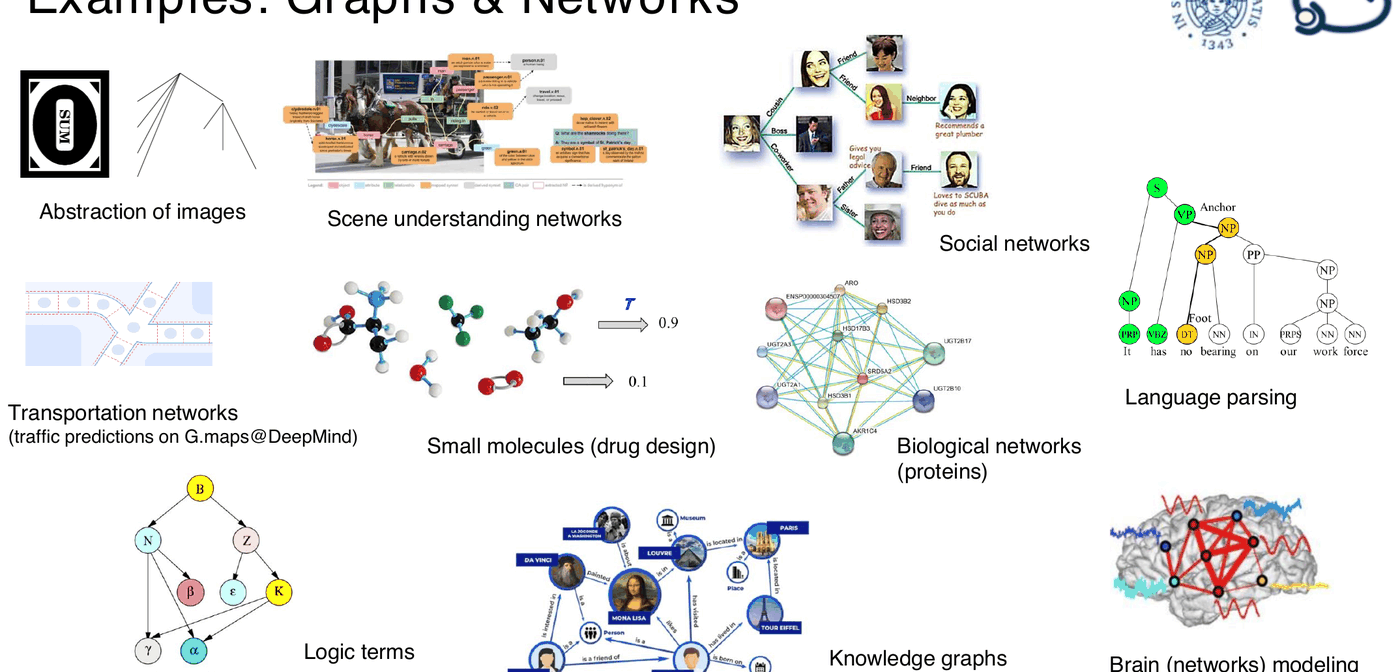
\includegraphics[width=0.91\linewidth,height=0.42\textheight,keepaspectratio]{images/21-sdl_esempi-grafi.png}
\caption{Examples of graphs and networks in different domains.}
\end{figure}

\subsection{The scenario}\label{lo-scenario}

\begin{figure}[htbp]
\centering
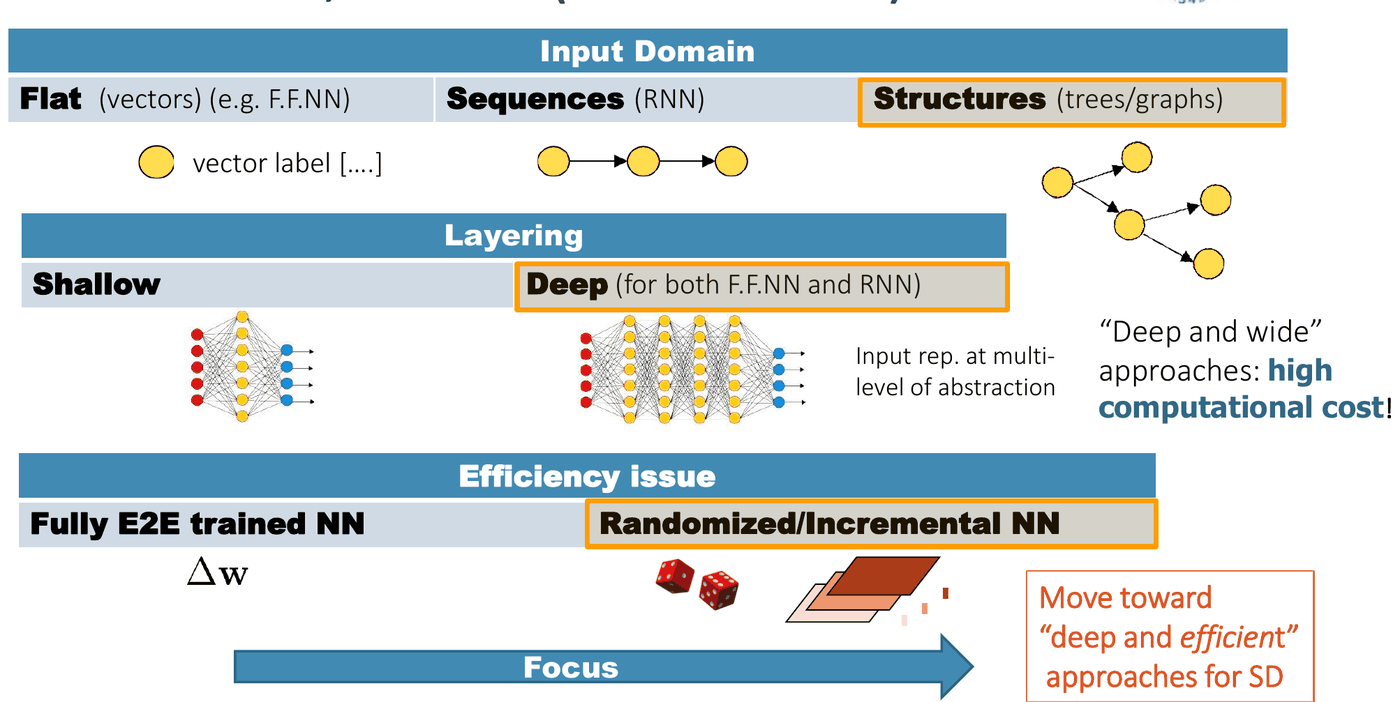
\includegraphics[width=0.89\linewidth,height=0.42\textheight,keepaspectratio]{images/21-sdl_scenario.png}
\caption{The scenario: from flat to structured input domains, from
shallow to deep models, from end-to-end to randomised or incremental
training. The goal is to obtain ``deep and efficient'' approaches for
structured data.}
\end{figure}

The course has followed this progression: from \textbf{vectors}
(feedforward networks) to \textbf{sequences} (RNNs) to
\textbf{structures} (trees, graphs). Deep and ``wide'' (\emph{deep and
wide}) approaches represent the input at several levels of abstraction
but have a high computational cost; \textbf{randomised} or
\textbf{incremental} networks offer efficiency.

\subsection{A bit of history}\label{un-po-di-storia}

Neural networks for structured data have a largely \textbf{Italian}
history:

\begin{itemize}
\tightlist
\item
  since the late 1990s, \textbf{recursive neural networks} for trees
  and directed acyclic graphs (Sperduti, Starita, Frasconi, Gori,
  Hammer, Micheli, Bianchini, Scarselli, Hagenbuchner\ldots): recursive
  networks (1997--2000), Cascade Correlation for structures, SOMs for
  structures (2003--2005), bottom-up Hidden Tree Markov Models (2012),
  Tree ESN and deep reservoir computing for trees (2010--2018);
\item
  the extension to \textbf{general graphs}, pioneered between Pisa and
  Siena (2005--2009), with two approaches:

  \begin{enumerate}
  \def\labelenumi{\arabic{enumi}.}
  \tightlist
  \item
    \textbf{recursive}: \textbf{GNN} (Scarselli et al., 2009) and
    \textbf{GraphESN} (Gallicchio, Micheli, 2010);
  \item
    \textbf{layered / convolutional}: \textbf{NN4G} (Micheli, 2009) in
    a constructive version, later continued as convolutional networks
    for graphs (GCN, etc.).
  \end{enumerate}
\end{itemize}

Since 2015 it has been an \textbf{exploding} area worldwide, with dozens
of papers at all the main conferences and real applications, under
different names: \emph{Graph Representation Learning}, \emph{learning on
graphs}, \emph{deep learning for graphs}, \emph{Graph Neural Networks}
(GNN), \emph{Graph Convolutional Networks} (GCN), and the framework of
\textbf{Deep Graph Networks} (DGN; Bacciu, Errica, Micheli, Podda,
2020).

\section{Deep Graph Networks}\label{deep-graph-networks}

\subsection{The graphs considered}\label{i-grafi-considerati}

We consider \textbf{labelled graphs}: each \textbf{node} (vertex) \(v\)
has a \textbf{vector label} \(\mathbf{l}(v)\) (e.g.\
\([1, 0, 1, 0.7]\)), each \textbf{edge} (link) can have a label (e.g.\
a position) and can be directed; there can be \textbf{cycles}. \(A\) is
the \textbf{adjacency matrix} of the graph.

\begin{figure}[htbp]
\centering
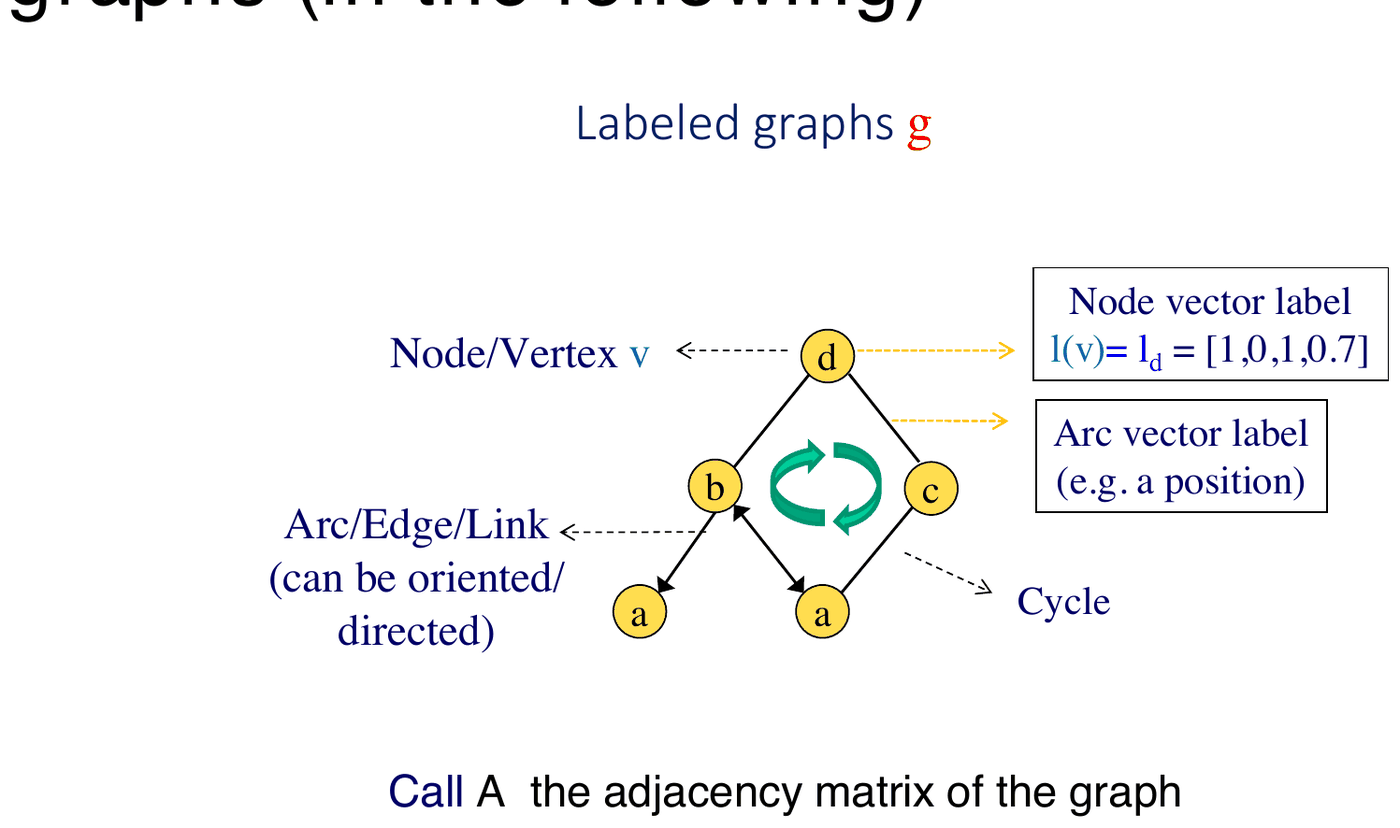
\includegraphics[width=0.63\linewidth,height=0.42\textheight,keepaspectratio]{images/21-sdl_grafo-etichettato.png}
\caption{A labelled graph: vector labels on nodes and edges, possible
cycles.}
\end{figure}

\subsection{The representation
problem}\label{il-problema-della-rappresentazione}

There was no \textbf{systematic} way (valid for any task) to extract
features or relationship metrics between structured examples. It is an
instance of \textbf{representation learning}, extended to structured
domains.

\begin{itemize}
\tightlist
\item
  \textbf{Feature}-based representations are incomplete or strongly
  task-dependent (for example topological indices in chemistry).
\item
  Representations with \textbf{adjacency matrices} or other fixed-size
  representations have problems: over-sizing or incompleteness (waste
  with padding or loss of information), \textbf{alignment} between
  different graphs (which node of one graph corresponds to which node
  of the other?), topological order (which makes generalisation
  difficult).
\end{itemize}

\begin{boxtip}{Moving the models towards the data}

\emph{``The ability to treat the inherent nature of the input data is
the key to a successful application of ML methodologies.''} Instead of
\textbf{bringing the data to the models} (turning graphs into vectors or
trees into sequences, with alignment problems and loss of information),
one \textbf{brings the models to the data}.

\end{boxtip}

\begin{boxexample}{Molecules and transductions}

In \textbf{QSPR/QSAR} one wants to correlate the chemical structure of
molecules with their properties:
\(\text{Property/Activity} = T(\text{Structure})\), a property value
(regression) or ``toxic yes/no'' (classification). Molecules \textbf{are
not vectors}: they are more naturally represented by variable-size
structures. Can we predict directly from the structures?

\end{boxexample}

\subsection{Transductions on graphs}\label{trasduzioni-su-grafi}

The goal is to learn a \textbf{transduction} \(T\) from a structured
domain to a discrete or continuous space, starting from examples
\((\text{graph}_i, \text{target}_i)\) with variable-size graphs.

\begin{figure}[htbp]
\centering
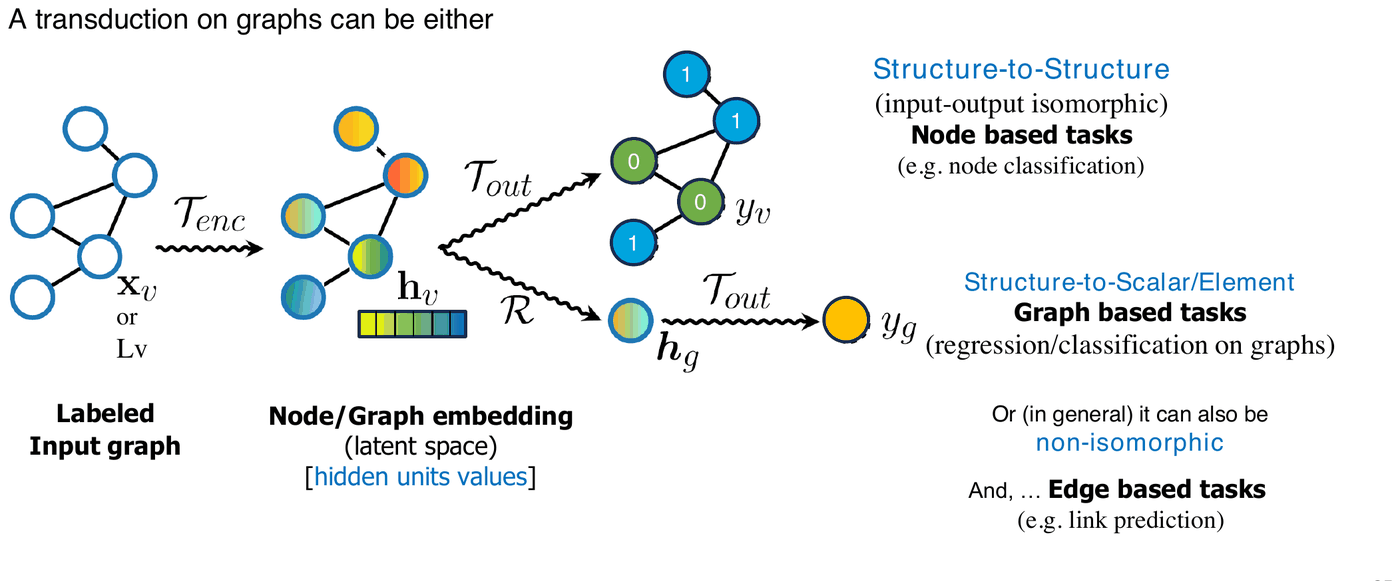
\includegraphics[width=0.89\linewidth,height=0.42\textheight,keepaspectratio]{images/21-sdl_trasduzioni.png}
\caption{Transductions on graphs: the graph is encoded into a node
embedding, from which per-node or whole-graph outputs are obtained.}
\end{figure}

\begin{itemize}
\tightlist
\item
  \textbf{Structure → structure} (input-output isomorphic):
  \textbf{node-level} tasks (e.g.\ node classification).
\item
  \textbf{Structure → scalar/element}: \textbf{graph-level} tasks
  (graph regression or classification).
\item
  In general also non-isomorphic; and \textbf{edge-level} tasks
  (e.g.\ \emph{link prediction}).
\end{itemize}

\subsection{Message passing}\label{il-message-passing}

How does a DGN work? The abstract concept is \textbf{message passing}:
nodes ``talk'' to each other, exchanging messages to inform one another
and become aware of the surrounding structure.

\begin{enumerate}
\def\labelenumi{\arabic{enumi}.}
\tightlist
\item
  Each node computes a \textbf{message}, a function of its own label,
  of its neighbours \(\mathcal{N}_v\) and of the edges between them,
  and sends it to its neighbours.
\item
  Nodes \textbf{aggregate} the received messages with a
  \textbf{permutation-invariant} function (the order in which they
  arrive does not matter).
\item
  Each node \textbf{updates} its own attributes (the \textbf{state}) by
  combining the messages with the free parameters \(W\).
\end{enumerate}

\begin{figure}[htbp]
\centering
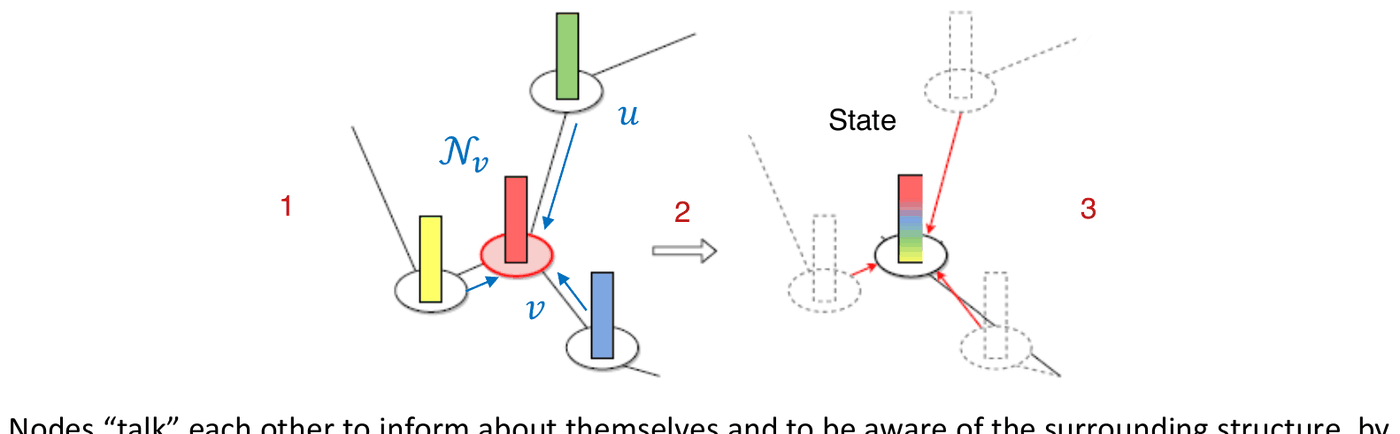
\includegraphics[width=0.80\linewidth,height=0.42\textheight,keepaspectratio]{images/21-sdl_message-passing.png}
\caption{Message passing: messages from neighbours, aggregation, state
update.}
\end{figure}

The state does not depend only on the local neighbourhood:
\textbf{iterating} message passing, information \textbf{spreads} from
each node to all the others. Finally, an output can be emitted
\textbf{for each node}, or \textbf{for the whole graph} through a
permutation-invariant aggregation of the node representations, called
\textbf{global pooling} (for example sum or mean).

\subsection{The link with CNNs}\label{il-legame-con-le-cnn}

Both CNNs and convolutional networks for graphs visit each node of the
data, but:

\begin{itemize}
\tightlist
\item
  in the \textbf{CNN} the convolutional kernel is applied on a
  \textbf{regular} 2D \textbf{grid}: a weighted average of the pixels in
  the window is computed, and the neighbours of a pixel are
  \textbf{ordered} and \textbf{fixed in number};
\item
  on \textbf{graphs} the CNN cannot be applied directly: the neighbours
  of a vertex are \textbf{unordered} and \textbf{variable in number}.
  The receptive field is limited to the \textbf{neighbours},
  \textbf{weight sharing} is used in a permutation-invariant way
  (abstracting from any node ordering), and the local neighbourhood is
  extended through \textbf{layering}.
\end{itemize}

\begin{figure}[htbp]
\centering
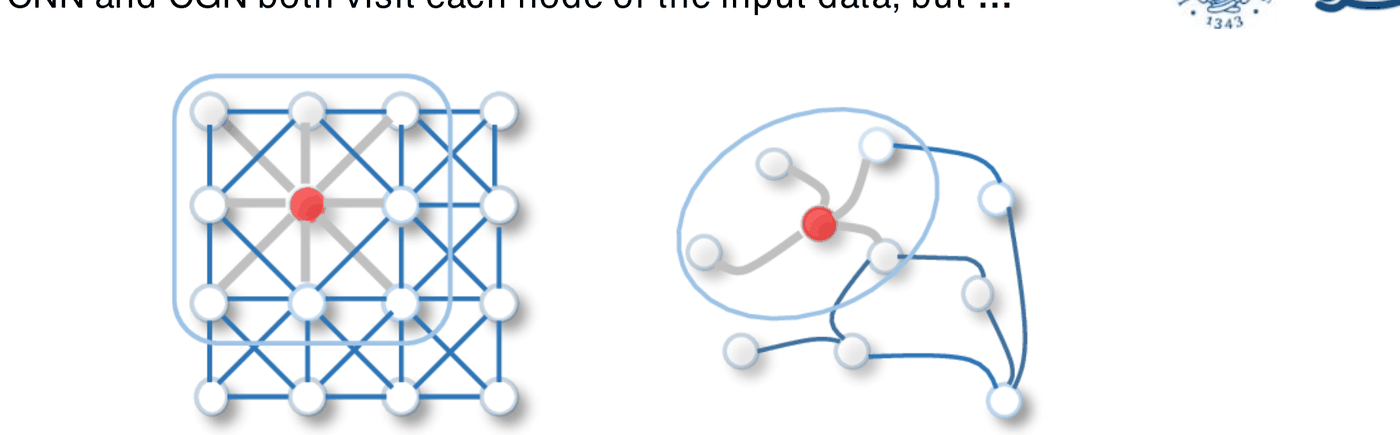
\includegraphics[width=0.80\linewidth,height=0.42\textheight,keepaspectratio]{images/21-sdl_cnn-vs-grafi.png}
\caption{Convolution on a grid (CNN) and on a graph.}
\end{figure}

\subsection{The general formula}\label{la-formula-generale}

Message passing is iterated over layers (or iterations) \(l\): \[
\mathbf{h}_v^{(l)} = AGG_{W^{(l)}}\Big(\mathbf{L}_v,\; \mathbf{h}_v^{(l-1)},\; \{\mathbf{h}_u^{(l-1)} : u \in \mathcal{N}(v)\}\Big), \qquad l = 1, \dots, L,
\] where \(AGG\) aggregates (propagates) the messages from the
neighbours \(u\) with a \textbf{permutation-invariant} operator over the
set of neighbours (e.g.\ a sum) and combinations of the unit
activations, \(W\) are the free parameters, \(\mathbf{L}_v\) is the
node label, and \(\mathcal{N}\) is given by the adjacency matrix \(A\).
Applying this computation to each node corresponds to a
\textbf{parallel, unordered visit} of the graph at each iteration.

There are many variants:

\begin{itemize}
\tightlist
\item
  \textbf{GCN} (Kipf, Welling, 2017):
  \(\mathbf{h}^{(l)} = \text{ReLU}\big(\hat{A}\,\mathbf{h}^{(l-1)}W^{(l)}\big)\),
  with \(\hat A\) the degree-normalised adjacency matrix;
\item
  \textbf{GraphConv} (Morris et al., 2019):
  \(\mathbf{h}^{(l)} = f\big(W_1^{(l)}\mathbf{h}^{(l-1)} + W_2^{(l)}A\,\mathbf{h}^{(l-1)}\big)\);
\item
  \textbf{GAT} (Veličković et al., 2018): \textbf{attention}-based
  aggregation.
\end{itemize}

(Many are available in \emph{PyTorch Geometric}.)

\begin{boxtip}{Why it is relevant for deep learning}

DGNs are \textbf{intrinsically deep}: the process is not local.
Iterating over the layers, the latent representations of the nodes
progressively include the \textbf{contextual} information of
increasingly distant nodes (diffusion).

\end{boxtip}

\begin{figure}[htbp]
\centering
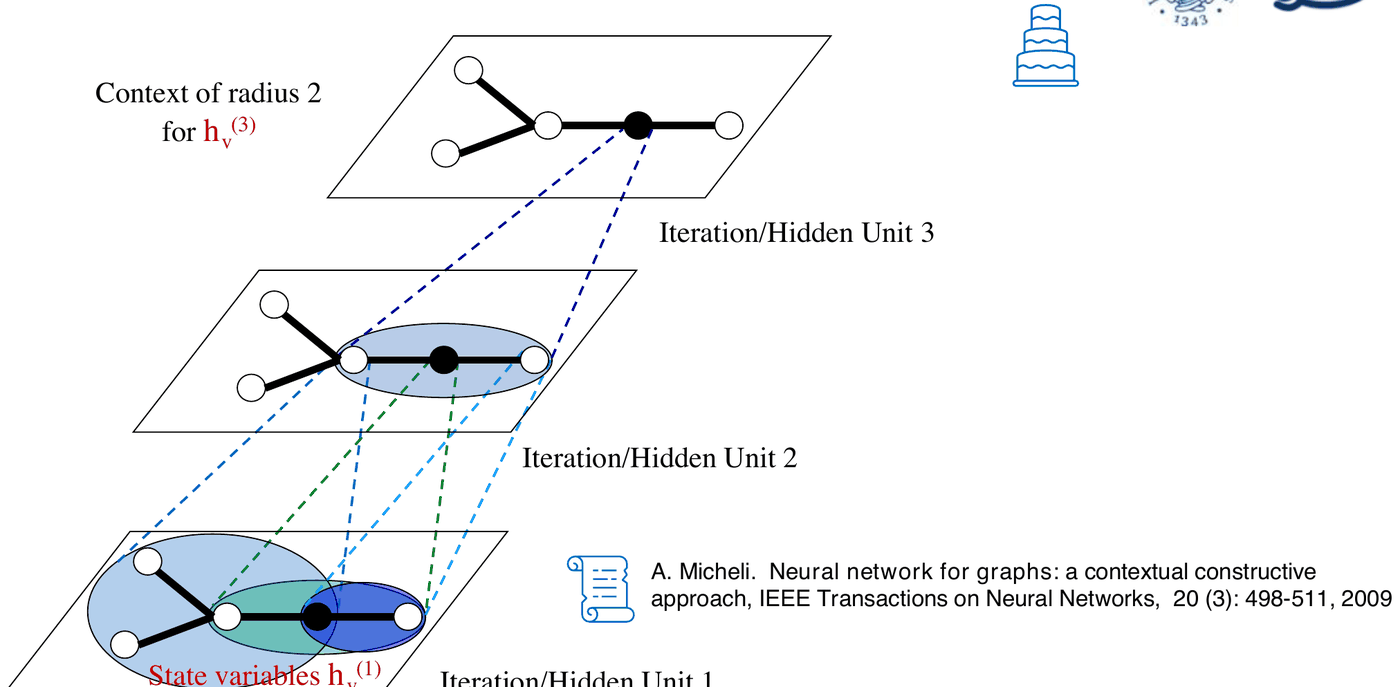
\includegraphics[width=0.86\linewidth,height=0.42\textheight,keepaspectratio]{images/21-sdl_contesto.png}
\caption{Evolution of the (compositional) context through the
iterations: at the third layer the state of the node has a context of
radius 2.}
\end{figure}

\subsection{NN4G and GCN: iterations as
layers}\label{nn4g-e-gcn-iterazioni-come-strati}

\begin{figure}[htbp]
\centering
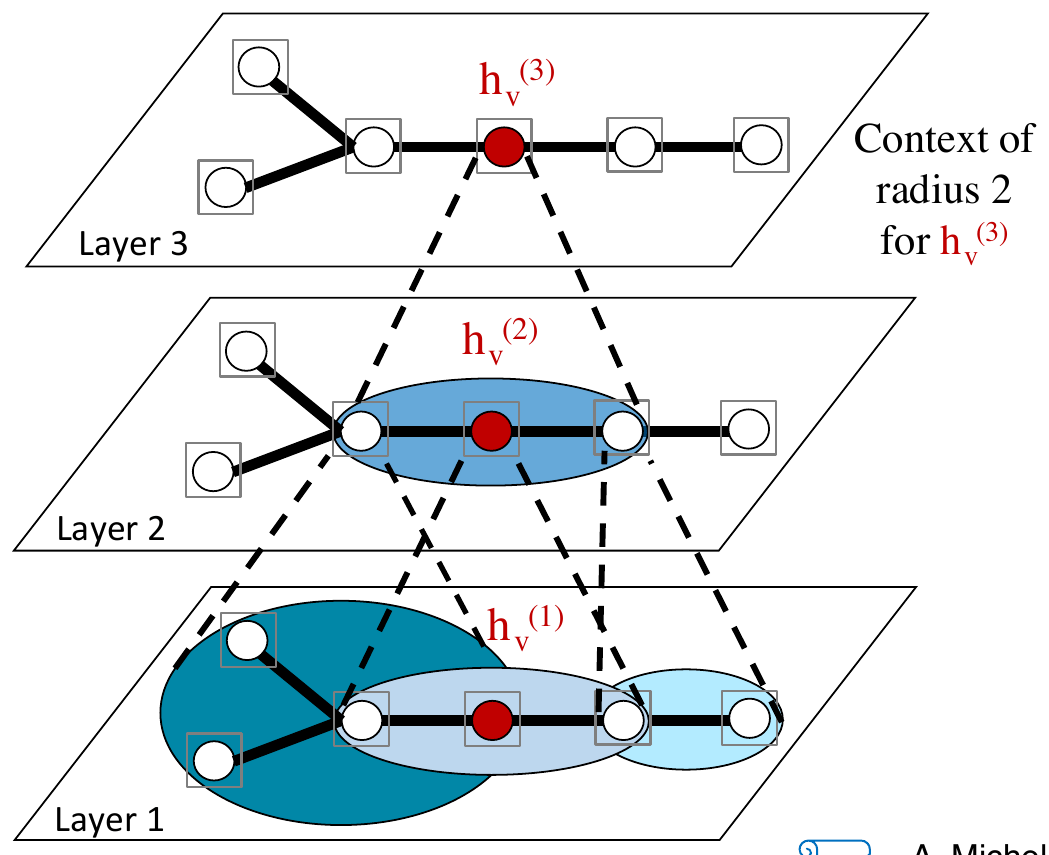
\includegraphics[width=0.49\linewidth,height=0.42\textheight,keepaspectratio]{images/21-sdl_nn4g.png}
\caption{GCN and NN4G: each message passing iteration is a new layer.}
\end{figure}

In convolutional networks for graphs (GCN, NN4G), \textbf{each message
passing iteration is a new layer}, and for each node the context is
\textbf{composed} across the layers:

\begin{itemize}
\tightlist
\item
  the \textbf{receptive field} extends incrementally as the layers
  increase;
\item
  \textbf{depth serves the growth of the context};
\item
  by training the model one learns \textbf{how to represent the graph}:
  end-to-end for general GCNs, \textbf{layer by layer} (incrementally)
  for NN4G, with an automatic number of layers and without vanishing
  gradient problems.
\end{itemize}

\textbf{NN4G} (Micheli, 2009) computes a state variable for each layer
and each vertex: \[
h_v^{(1)} = f\left(\sum_{j=0}^{|L_v|}\bar w_{1j}\,L_j(v)\right), \qquad h_v^{(l)} = f\left(\underbrace{\sum_{j=0}^{|L_v|}\bar w_{lj}\,L_j(v)}_{\text{label of } v} + \underbrace{\sum_{j=1}^{l-1}\hat w_{lj}\sum_{u \in \mathcal{N}(v)}h_u^{(j)}}_{\text{context from neighbours, from all previous layers}}\right), \quad l = 2, \dots, N.
\] It is not recursive: each layer uses the states of the
\textbf{previous} layers. Units are added one at a time (in Cascade
Correlation style), and the outputs of the various layers are combined
to produce the result on the graph.

\subsection{GNN and GraphESN: recursive
approach}\label{gnn-e-graphesn-approccio-ricorsivo}

In \textbf{recursive} approaches (GNN, GraphESN) the diffusion process
is similar, but \(l\) is the number of \textbf{iterations on the same
layer} (or layers with shared weights). It is a \textbf{dynamical
system}: typically \textbf{convergence to a fixed point} is required,
used as the graph embedding, and for this reason the message passing
dynamics is constrained to be \textbf{contractive}.

\begin{itemize}
\tightlist
\item
  \textbf{GNN} (Scarselli et al., 2009): with training of the
  embedding.
\item
  \textbf{GraphESN} (Gallicchio, Micheli, 2010): it extends Echo State
  Networks: the message passing function \textbf{is not trained} (it is
  a random reservoir), but the parameters of the dynamical system are
  controlled directly.
\end{itemize}

\[
\mathbf{h}_v^{(l)} = \tanh\left(\sum_{j=0}^{|L_v|}\bar w_{lj}\,L_j(v) + \sum_{u \in \mathcal{N}(v)}\hat W\,\mathbf{h}_u^{(l-1)}\right),
\] iterated until convergence; the output for a graph is obtained with
a global pooling \(X\) and a \textbf{linear readout} trained with the
pseudoinverse or ridge regression: \(y(g) = W_{out}\,X(\mathbf{h}(g))\).

\begin{figure}[htbp]
\centering
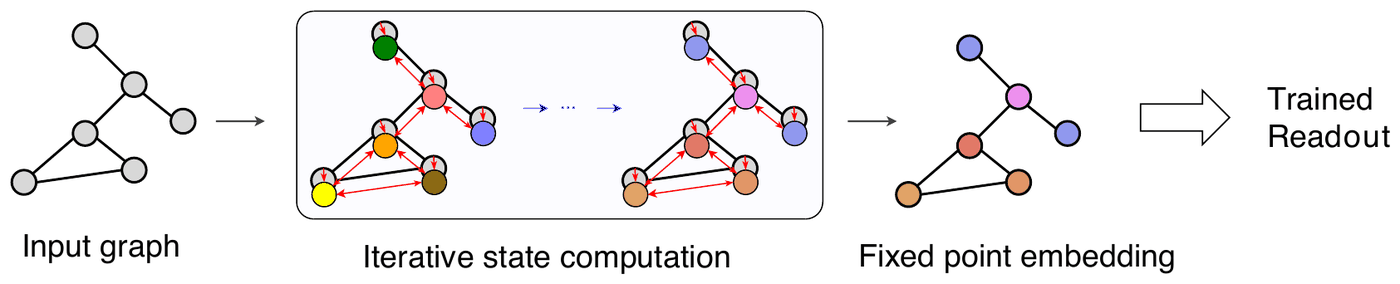
\includegraphics[width=0.80\linewidth,height=0.42\textheight,keepaspectratio]{images/21-sdl_gesn.png}
\caption{GraphESN: iterative computation of the states up to a
fixed-point embedding, then trained readout.}
\end{figure}

\section{Open problems and some
proposals}\label{problemi-aperti-e-alcune-proposte}

\begin{figure}[htbp]
\centering
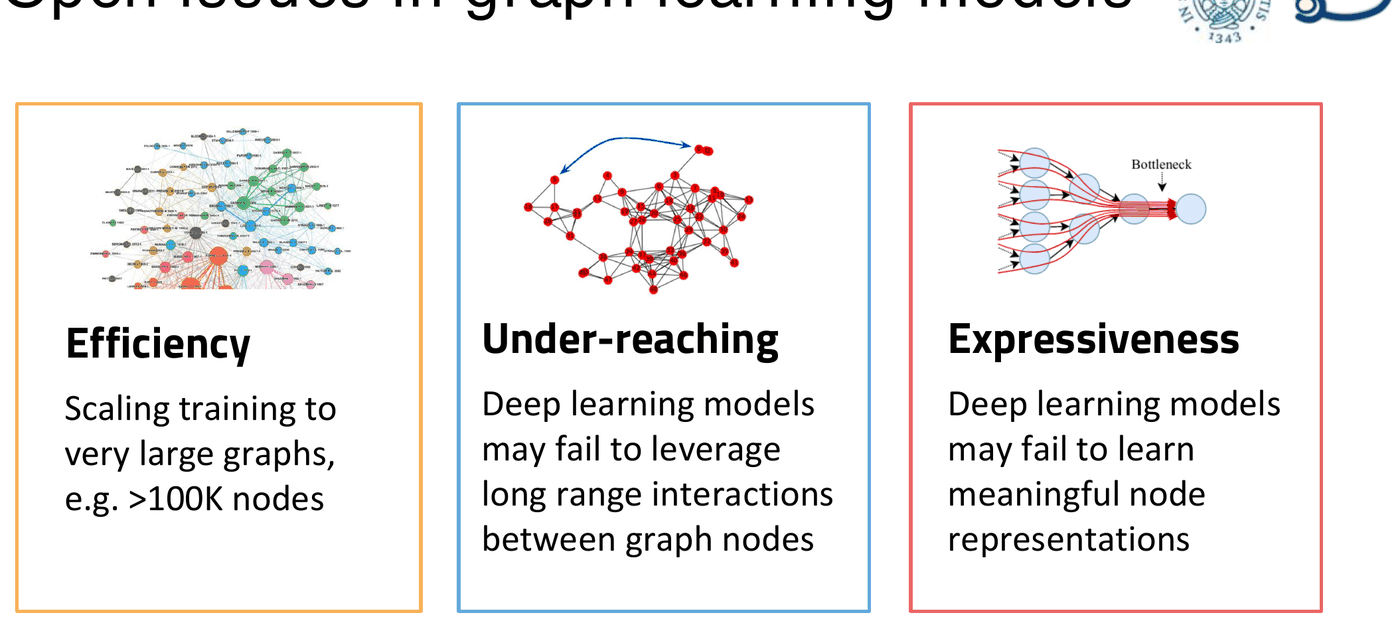
\includegraphics[width=0.86\linewidth,height=0.42\textheight,keepaspectratio]{images/21-sdl_problemi-aperti.png}
\caption{Open problems in graph learning models: efficiency,
under-reaching, expressiveness.}
\end{figure}

\subsection{Efficiency: beyond end-to-end
backpropagation}\label{efficienza-oltre-la-backpropagation-end-to-end}

\begin{itemize}
\tightlist
\item
  \textbf{GraphESN for node classification}: on very large graphs
  (e.g.\ Twitch-gamers, 168,000 nodes) it achieves accuracy equal to or
  higher than most end-to-end trained models, with a speed-up of up to
  10 times, and training scales easily beyond 100,000 nodes.
\item
  \textbf{NN4G+} (automatic architecture design): the network is built
  \textbf{incrementally}, with a synergistic double expansion. It is
  trained \textbf{one unit at a time} (no end-to-end backpropagation
  across layers); a layer is expanded as long as the validation
  accuracy improves, and new layers are added as long as it improves.
  The resulting architectures are adapted to the task, consistently
  deeper and leaner compared to an explicit architecture search, and
  they are built in minutes instead of hours (more than 10 times
  faster, without loss of accuracy).
\end{itemize}

\subsection{The problems of depth: the
``over-*''}\label{i-problemi-della-profondituxe0-gli-over-}

Depth is needed, but message passing has biases and problems:

\begin{itemize}
\tightlist
\item
  \textbf{Over-smoothing} (Li et al., 2018): accuracy typically drops
  beyond 4--5 layers; node representations \textbf{collapse} in the
  deep layers. Message passing acts as a \textbf{diffusion}, and the
  high-level representations of the nodes all become similar.
\item
  \textbf{Over-squashing} (Alon, Yahav, 2021): it is a
  \textbf{bottleneck}. The receptive field grows
  \textbf{exponentially} with depth, but all this information must be
  compressed into a fixed-size embedding per node. The
  \textbf{sensitivity} of a node's representation to the input features
  of distant nodes, measured by the Jacobian
  \(\partial\mathbf{h}_v^{(L)}/\partial\mathbf{x}_u\), decreases
  exponentially with the number of layers.
\item
  For end-to-end training, the \textbf{difficulty of backpropagating
  the gradient} through many message passing layers.
\end{itemize}

The interaction among these phenomena is an open research problem. The
effects:

\begin{enumerate}
\def\labelenumi{\arabic{enumi}.}
\tightlist
\item
  \textbf{Under-reaching}: the over-* prevent having the receptive
  field needed to learn interactions between distant nodes.
\item
  \textbf{Heterophily} in node classification. In \textbf{homophilous}
  graphs nodes in the same neighbourhood mostly share the same class;
  in \textbf{heterophilous} graphs nodes of the same class are
  generally far apart, and predictions based mainly on immediate
  neighbours can be misleading. These are potentially hard tasks for
  standard message passing, because of the over-* and the bias towards
  ``homogeneous'' graphs.
\end{enumerate}

\begin{figure}[htbp]
\centering
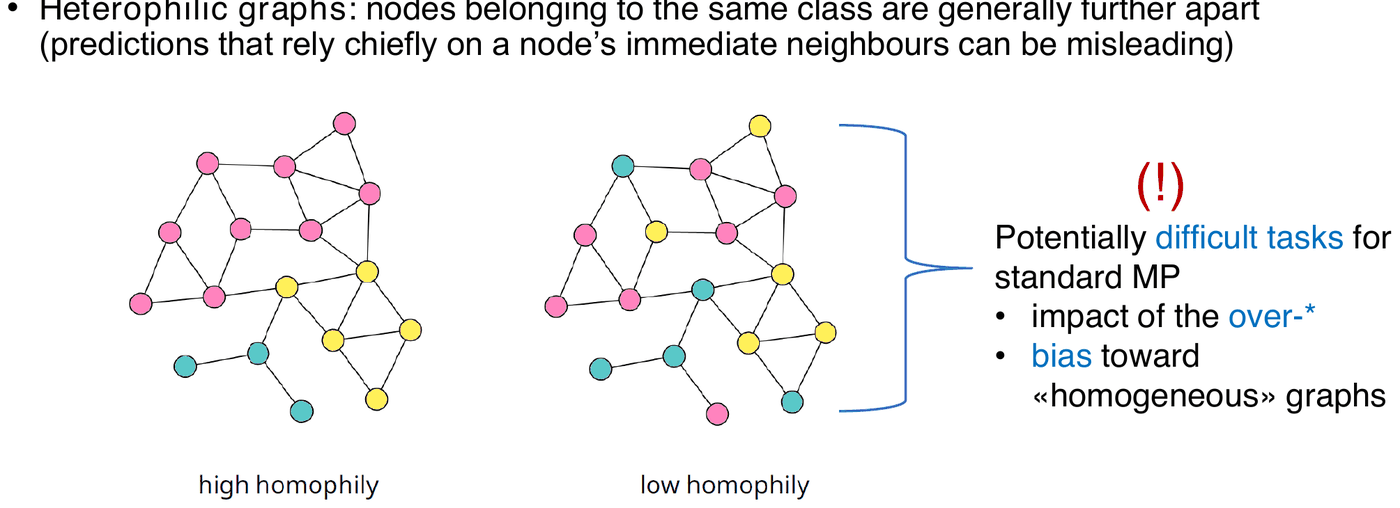
\includegraphics[width=0.80\linewidth,height=0.42\textheight,keepaspectratio]{images/21-sdl_eterofilia.png}
\caption{High- and low-homophily graphs: the latter are hard for standard
message passing.}
\end{figure}

\subsubsection{Analysis tools}\label{strumenti-per-lanalisi}

\begin{itemize}
\tightlist
\item
  \textbf{Models that separate the bias of message passing from the
  problems of end-to-end training}: NN4G (incremental, without
  propagating the gradient across layers) and GraphESN (no training of
  the embedding, direct control of the spectral norm \(\|W\|\), i.e.\
  of the Lipschitz constant of the recursive message passing function).
  Since \[
  \left\|\frac{\partial\mathbf{h}_v^{(L)}}{\partial\mathbf{x}_u}\right\| \le \prod_{l=1}^{L}\|W^{(l)}\|\cdot\big(A^L\big)_{u,v},
  \] imposing \(\|W\| > 1\) prevents the sensitivity with respect to
  the input from vanishing exponentially (over-squashing).
\item
  \textbf{Spectral analysis} of the layers. ``Frequency'' on a graph is
  the variability of the signal (labels, embeddings) between
  neighbouring nodes. The \textbf{Dirichlet energy}
  \(E(\mathbf{h}) = \sum_{v}\sum_{u \in \mathcal{N}_v}\|\mathbf{h}_v - \mathbf{h}_u\|^2\)
  measures how much the signal varies over the graph (spatial view)
  and, through the graph Fourier transform (obtained from the
  decomposition of the Laplacian \(L = D - A\)), how the ``mass'' of the
  signal is distributed over the frequency spectrum: a low-frequency
  (smooth) signal has low energy. Heterophilous graphs have
  \textbf{high-frequency} signals, and heterophilous tasks require
  \textbf{preserving high frequencies}.
\end{itemize}

On the \textbf{Chameleon} dataset (a network of Wikipedia pages, 2277
nodes, 31,400 edges, homophily 0.23), a ``stress test'' for
heterophily, NN4G and GraphESN \textbf{better preserve the energy}
across layers, and while the accuracy of the other models drops as
message passing increases, theirs does not. In an experiment with 12
layers: GraphESN 73.7\%, NN4G 68.3\%, GCN 57.8\%, GAT 55.0\%, GraphConv
33.8\%.

\subsection{Ongoing extensions}\label{estensioni-in-corso}

\begin{itemize}
\tightlist
\item
  \textbf{Dynamic/temporal graphs}: relationships or node values that
  evolve over time (spread of infections, content on social networks,
  signals on nodes). \textbf{Dynamic Graph Echo State Networks}
  implement a spatio-temporal convolution with a multi-layer reservoir,
  as effective as fully trained temporal graph networks, but with a
  100-fold speed-up in training and 10-fold in inference.
\item
  \textbf{Graph generation}: learning the distribution \(p(G)\) of a
  set of graphs in order to sample new ones (e.g.\ fragment-based
  molecule generation), useful for fairness, robustness, privacy.
\item
  \textbf{Explainability} (XAI) for graph networks: for example
  identifying the benzene rings that determine a classification, or the
  known structural fragments (such as the Michael acceptor) that affect
  the activation of the P53 pathway in the Tox21 data.
\item
  \textbf{Network quantification}: predicting the \textbf{prevalence}
  of the classes among the unlabelled nodes instead of classifying them
  individually (voting, market research, epidemiology).
\item
  \textbf{Bioinformatics}: predicting dynamic properties (robustness,
  sensitivity) of biochemical pathways and protein-protein interaction
  networks represented as graphs.
\end{itemize}

\section{Other approaches: kernels for
structures}\label{altri-approcci-i-kernel-per-strutture}

\textbf{Kernel methods} extend easily to graphs of different types
(sequences, trees, directed or undirected graphs, cyclic or acyclic),
because it is enough to define a dot product
\(k(x, x') = \langle\phi(x), \phi(x')\rangle\), i.e.\ a
\textbf{similarity} between data of any type, with an implicit
embedding in a Euclidean space.

\begin{itemize}
\tightlist
\item
  \textbf{Marginalised kernels}: the similarity between two graphs is
  based on the common label paths obtained with random walks; the
  kernel is the dot product of the count vectors, averaged over all
  possible paths. The cost typically scales quadratically with the size
  of the graph.
\item
  \textbf{Convolution kernels}: objects are decomposed into
  \textbf{sub-structures} and the kernel is defined by combining
  kernels between the sub-structures.
\end{itemize}

\begin{figure}[htbp]
\centering
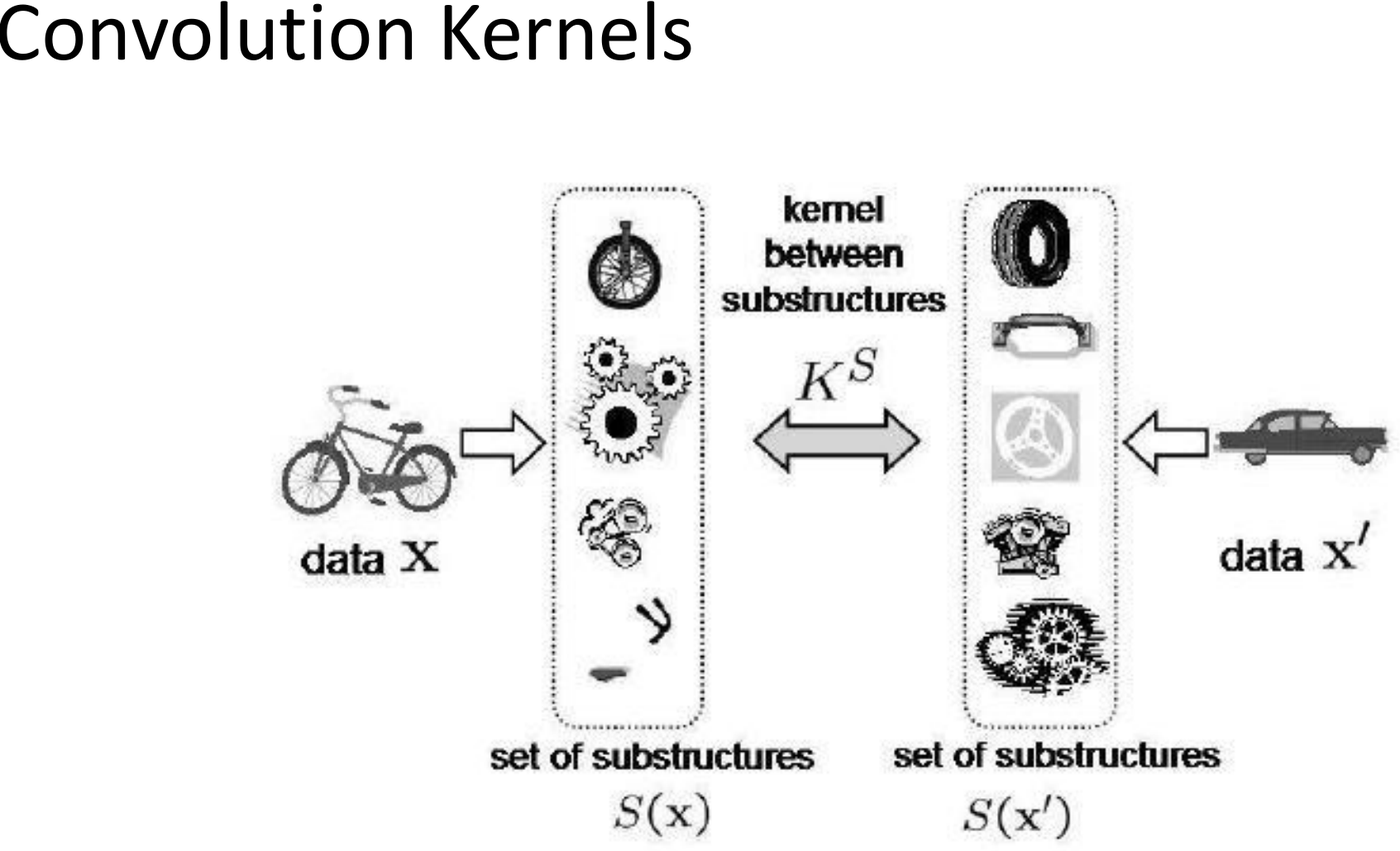
\includegraphics[width=0.63\linewidth,height=0.42\textheight,keepaspectratio]{images/21-sdl_convolution-kernel.png}
\caption{Convolution kernel: the similarity between objects is computed
from the similarity between their sub-structures.}
\end{figure}

\begin{boxwarning}{Limits of kernels for structures}

\begin{itemize}
\tightlist
\item
  \textbf{Efficiency}: the cost is critical, because of the
  decomposition into sub-structures.
\item
  \textbf{Adaptivity}: they are knowledge-driven methods, with a
  similarity measure \textbf{fixed before learning}: the encoding in the
  feature space is not learned. The advantage is being able to exploit
  prior knowledge for a specific problem.
\item
  For structured domains \textbf{universality is not known}: the choice
  of the kernel is critical, and computing a \textbf{complete} kernel
  for graphs is at least as hard as the \textbf{graph isomorphism}
  problem. (Adaptive kernels are being studied.)
\end{itemize}

\end{boxwarning}

\begin{boxabstract}{Conclusions}

\begin{itemize}
\tightlist
\item
  Deep learning on complex data can be done \textbf{efficiently},
  without fully end-to-end training: models such as GraphESN and NN4G
  build accurate DGNs efficiently and make it possible to study the
  bias of message passing.
\item
  \textbf{Depth} in DGNs is necessary (it makes the context grow), but
  it can cause problems (over-smoothing, over-squashing, training
  difficulties); going beyond end-to-end can help both for efficiency
  and for the over-*.
\item
  ML for structured data and graphs is a concrete reality, still under
  development, that offers new solutions where \textbf{relationships}
  matter. If the data have relationships (serial, hierarchical,
  networks), \textbf{it is not advisable to use a flat
  representation}. It is also a great opportunity to treat different
  data types uniformly.
\end{itemize}

\end{boxabstract}

\begin{boxquestion}{Possible exam questions}

\begin{itemize}
\tightlist
\item
  Why treat structured data directly, instead of turning them into
  vectors?
\item
  Which types of transduction can be defined on graphs?
\item
  Describe message passing and the general formula of DGNs.
\item
  Difference between layered (GCN, NN4G) and recursive (GNN, GraphESN)
  approaches.
\item
  What are over-smoothing and over-squashing? What is heterophily?
\item
  Pros and cons of kernels for structures.
\end{itemize}

\end{boxquestion}
